%%%%%%%%%%%%%%%%%%%%%%%%%%%%%%%%%%%%%%%%%
% Beamer Presentation
% LaTeX Template
% Version 1.0 (10/11/12)
%
% This template has been downloaded from:
% http://www.LaTeXTemplates.com
%
% License:
% CC BY-NC-SA 3.0 (http://creativecommons.org/licenses/by-nc-sa/3.0/)
%
%%%%%%%%%%%%%%%%%%%%%%%%%%%%%%%%%%%%%%%%%

%----------------------------------------------------------------------------------------
%	PACKAGES AND THEMES
%----------------------------------------------------------------------------------------

\documentclass{beamer}

\mode<presentation> {

% The Beamer class comes with a number of default slide themes
% which change the colors and layouts of slides. Below this is a list
% of all the themes, uncomment each in turn to see what they look like.

%\usetheme{default}
%\usetheme{AnnArbor}
%\usetheme{Antibes}
%\usetheme{Bergen}
%\usetheme{Berkeley}
%\usetheme{Berlin}
%\usetheme{Boadilla}
%\usetheme{CambridgeUS}
%\usetheme{Copenhagen}
%\usetheme{Darmstadt}
%\usetheme{Dresden}
%\usetheme{Frankfurt}
%\usetheme{Goettingen}
%\usetheme{Hannover}punto
%\usetheme{Ilmenau}
%\usetheme{JuanLesPins}punto
%\usetheme{Luebeck}
%\usetheme{Madrid}punto
%\usetheme{Malmoe}
%\usetheme{Marburg}
%\usetheme{Montpellier}punto
%\usetheme{PaloAlto}punto
%\usetheme{Pittsburgh}punto
%\usetheme{Rochester}punto
\usetheme{Singapore}
%\usetheme{Szeged}
%\usetheme{Warsaw}

% As well as themes, the Beamer class has a number of color themes
% for any slide theme. Uncomment each of these in turn to see how it
% changes the colors of your current slide theme.

%\usecolortheme{albatross}fondo azul
%\usecolortheme{beaver}titulos rojos
%\usecolortheme{beetle}fondo gris
%\usecolortheme{crane} resaltado amarillo
%\usecolortheme{dolphin} titulos azules
%\usecolortheme{dove} titulos negros
%\usecolortheme{fly} fondo gris, titulos blancos
%\usecolortheme{lily} ??
%\usecolortheme{orchid} ??
\usecolortheme{rose} %punto
%\usecolortheme{seagull} adornos gris
%\usecolortheme{seahorse} partes gris
%\usecolortheme{whale} partes azul
%\usecolortheme{wolverine} resalto amarillo

%\setbeamertemplate{footline} % To remove the footer line in all slides uncomment this line
\setbeamertemplate{footline}[page number] % To replace the footer line in all slides with a simple slide count uncomment this line

\setbeamertemplate{navigation symbols}{} % To remove the navigation symbols from the bottom of all slides uncomment this line
}

\usepackage{graphicx} % Allows including images
\usepackage{booktabs} % Allows the use of \toprule, \midrule and \bottomrule in tables
\usepackage{listings}
\usepackage{xcolor}

\colorlet{punct}{red!60!black}
\definecolor{background}{HTML}{EEEEEE}
\definecolor{delim}{RGB}{20,105,176}
\colorlet{numb}{magenta!60!black}

\lstdefinelanguage{json}{
    basicstyle=\normalfont\ttfamily,
    numbers=left,
    numberstyle=\scriptsize,
    stepnumber=1,
    numbersep=8pt,
    showstringspaces=false,
    breaklines=true,
    frame=lines,
    backgroundcolor=\color{background},
    literate=
     *{0}{{{\color{numb}0}}}{1}
      {1}{{{\color{numb}1}}}{1}
      {2}{{{\color{numb}2}}}{1}
      {3}{{{\color{numb}3}}}{1}
      {4}{{{\color{numb}4}}}{1}
      {5}{{{\color{numb}5}}}{1}
      {6}{{{\color{numb}6}}}{1}
      {7}{{{\color{numb}7}}}{1}
      {8}{{{\color{numb}8}}}{1}
      {9}{{{\color{numb}9}}}{1}
      {:}{{{\color{punct}{:}}}}{1}
      {,}{{{\color{punct}{,}}}}{1}
      {\{}{{{\color{delim}{\{}}}}{1}
      {\}}{{{\color{delim}{\}}}}}{1}
      {[}{{{\color{delim}{[}}}}{1}
      {]}{{{\color{delim}{]}}}}{1},
}
%----------------------------------------------------------------------------------------
%	TITLE PAGE
%----------------------------------------------------------------------------------------

\title[@MongoDB]{@MongoDB - Database No Only SQL} % The short title appears at the bottom of every slide, the full title is only on the title page

\author{jesse cogollo} % Your name
\institute[SENA] % Your institution as it will appear on the bottom of every slide, may be shorthand to save space
{
Developer by passion \\ % Your institution for the title page
\medskip
\textit{email: cogollo87@gmail.com} % Your email address
}
\date{\today} % Date, can be changed to a custom date

\begin{document}

\begin{frame}
\titlepage % Print the title page as the first slide
\end{frame}

\begin{frame}
\frametitle{Contenido} % Table of contents slide, comment this block out to remove it
\tableofcontents % Throughout your presentation, if you choose to use \section{} and \subsection{} commands, these will automatically be printed on this slide as an overview of your presentation
\end{frame}

%----------------------------------------------------------------------------------------
%	PRESENTATION SLIDES
%----------------------------------------------------------------------------------------

%------------------------------------------------
\section{MongoDB} % Sections can be created in order to organize your presentation into discrete blocks, all sections and subsections are automatically printed in the table of contents as an overview of the talk
%------------------------------------------------

\begin{frame}[fragile] % Need to use the fragile option when verbatim is used in the slide
\frametitle{Presentaci\'on}
\begin{example}[yo]

\begin{lstlisting}[language=json,firstnumber=1]
{
  "name": "Jesse Javier Cogollo Alvarez",
  "age": 27,
  "title": "Developer by passion",
  "location": "Medellin, Colombia",
  "phone": "3207906256",
  "Marital status": "Married",
  "member": ["@avanet","@MongoDBMedelln"],
  "social": {
    		"facebook": "jessecogollo", 
    		"skype": "jessecogollo", 
    		"twitter": ["@jessecogollo","@newdevs"]
  }
}
\end{lstlisting}

\end{example}
\end{frame}

%------------------------------------------------
\begin{frame}
\frametitle{Que es @MongoDB}
'MongoDB (from "humongous") is an open-source document database, and the leading NoSQL database. Written in C++.'
{\color{blue}\url{https://www.mongodb.org/}}
\\~\\
'MongoDB was not designed in a lab. We built MongoDB from our own experiences building large-scale,high availability, robust systems...'
\underline{\color{green}Eliot Horowitz, CTO and Co-Founder}	
\end{frame}

%------------------------------------------------

\begin{frame}
\frametitle{NOSQL}
“En inform\'atica, NoSQL (a veces llamado 'no só\'olo SQL') es una amplia clase de sistemas de gesti\'on de bases de datos que difieren del modelo cl\'asico del sistema de gesti\'on de bases de datos relacionales (RDBMS) en aspectos importantes, el m\'as destacado que no usan SQL como el principal lenguaje de consultas.” {\color{blue}\url{http://es.wikipedia.org/wiki/NoSQL/}}
\\~\\

\end{frame}

%------------------------------------------------

\begin{frame}
\frametitle{NOSQL}
Las caracteristicas comunes de las bases de datos NoSQL son:
\begin{itemize}
\item No utilizan el modelo relacional.
\item Corren bien en clusters.
\item Open-source.
\item sin esquemas.
\item El resultado mas importante del aumento de las bases de datos NoSQL es la {\color{green}Persistencia Poliglota}.
\end{itemize}
{\color{blue}\url{http://martinfowler.com/articles/nosqlKeyPoints.html}}
\end{frame}

%------------------------------------------------

\begin{frame}
\frametitle{Persistencia poliglota}
\begin{figure}
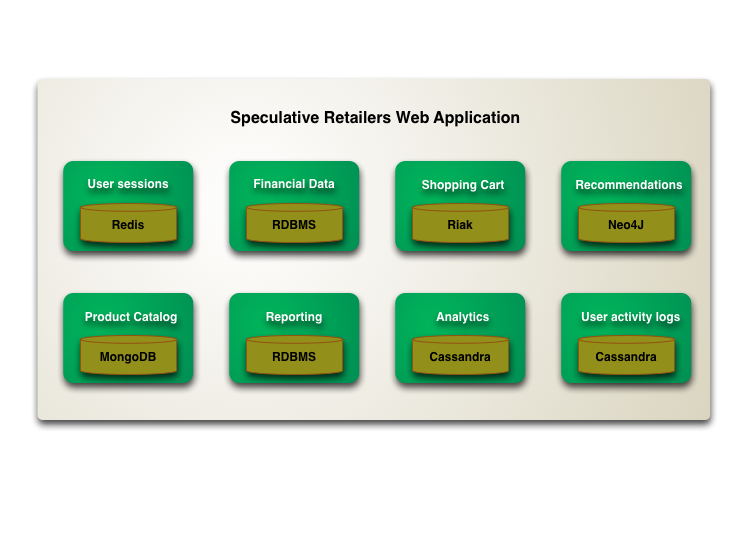
\includegraphics[width=1.0\linewidth]{polyglot.png}
\end{figure}
\end{frame}

%------------------------------------------------

\begin{frame}
\frametitle{JSON}
\begin{block}{Definici\'on}
 (JavaScript Object Notation) Formato de intercambio de datos.
\end{block}

\begin{block}{Esquema}
\begin{figure}
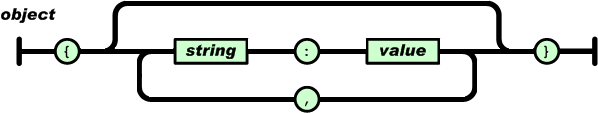
\includegraphics[width=0.7\linewidth]{object.png}
\end{figure}
\end{block}

\begin{block}{Ejemplo}
\begin{center}
\{ "llave": "valor" \} \'o \{\}
\end{center}
\end{block}
\end{frame}

%------------------------------------------------

\begin{frame}
\frametitle{JSON}
\begin{block}{Definici\'on array}
 Es el tipo de dato que puede contener un JSON.
\end{block}

\begin{block}{Esquema}
\begin{figure}
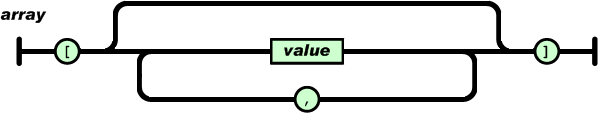
\includegraphics[width=0.7\linewidth]{array.png}
\end{figure}
\end{block}

\begin{block}{Ejemplo}
\begin{center}
["valor1", "sena",2014,true]
\end{center}
\end{block}

\end{frame}

%------------------------------------------------

\begin{frame}
\frametitle{JSON}
\begin{block}{Definici\'on valor}
 Es el tipo de dato que puede contener un JSON.
\end{block}

\begin{block}{value}
\begin{figure}
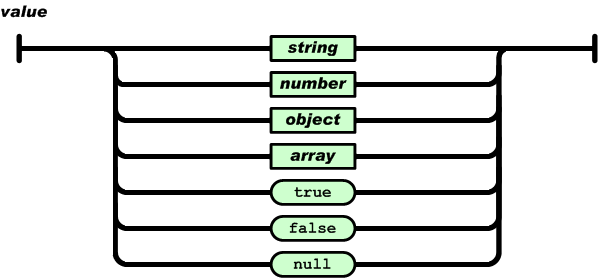
\includegraphics[width=0.7\linewidth]{value.png}
\end{figure}
\end{block}

\end{frame}

%------------------------------------------------

\begin{frame}
\frametitle{JSON}
\begin{block}{Esquema string}
\begin{figure}
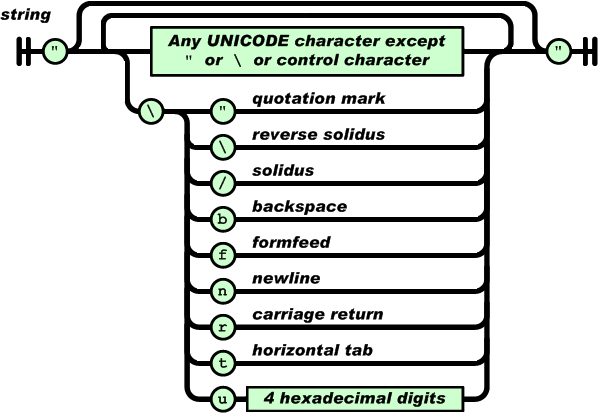
\includegraphics[width=0.7\linewidth]{string.png}
\end{figure}
\end{block}

\end{frame}

%------------------------------------------------


\begin{frame}
\frametitle{JSON}
\begin{block}{Esquema number}
\begin{figure}
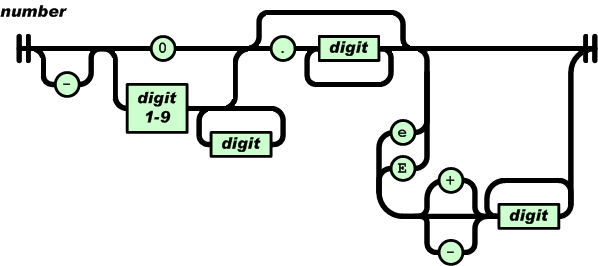
\includegraphics[width=0.7\linewidth]{number.png}
\end{figure}
\end{block}

\end{frame}

%------------------------------------------------
\begin{frame}
\frametitle{Caracteristicas}
\begin{columns}[c] % The "c" option specifies centered vertical alignment while the "t" option is used for top vertical alignment

\column{.45\textwidth} % Left column and width
\begin{enumerate}
\item \textbf{Document-Oriented Storage}
\item Full Index Support
\item Replication y High Availability
\item Auto Sharding
\item Querying
\item Map Reduce
\item GridFS
\item Other more...
\end{enumerate}

\column{.5\textwidth} % Right column and width
Las \textbf{colecciones} Son esquemas dinamicos, flexibles que ofrecen simplicidad y potencia.
\begin{figure}
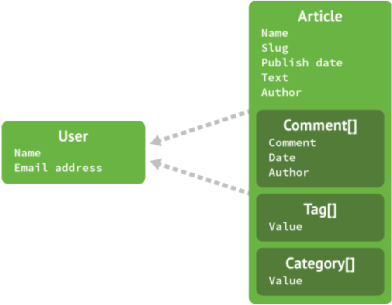
\includegraphics[width=0.9\linewidth]{document.png}
\end{figure}
\end{columns}
\end{frame}


%------------------------------------------------
\begin{frame}
\frametitle{Caracteristicas}
\begin{columns}[c] % The "c" option specifies centered vertical alignment while the "t" option is used for top vertical alignment

\column{.45\textwidth} % Left column and width
\begin{enumerate}
\item Document-Oriented Storage
\item \textbf{Full Index Support}
\item Replication y High Availability
\item Auto Sharding
\item Querying
\item Map Reduce
\item GridFS
\item Other more...
\end{enumerate}

\column{.5\textwidth} % Right column and width
Index provee alto desempeno en operaciones de lecturas.
\begin{figure}
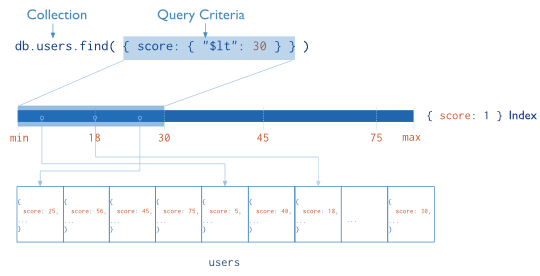
\includegraphics[width=1\linewidth]{index-with-query.png}
\end{figure}
MongoDB indexa utilizando estructura de datos B-tree.
\end{columns}
\end{frame}


%------------------------------------------------
\begin{frame}
\frametitle{Caracteristicas}
\begin{columns}[c] % The "c" option specifies centered vertical alignment while the "t" option is used for top vertical alignment

\column{.45\textwidth} % Left column and width
\begin{enumerate}
\item Document-Oriented Storage
\item Full Index Support
\item \textbf{Replication y High Availability}
\item Auto Sharding
\item Querying
\item Map Reduce
\item GridFS
\item Other more...
\end{enumerate}

\column{.5\textwidth} % Right column and width
replica set en MongoDB es un grupo de procesos mongod que mantienen el mismo conjunto de datos. provee redundancia y alta disponibilidad.
\begin{figure}
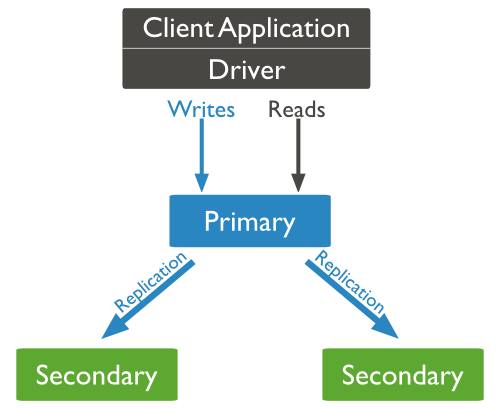
\includegraphics[width=0.6\linewidth]{replica-set-read-write-operations-primary.png}
\end{figure}
\end{columns}
\end{frame}


%------------------------------------------------
\begin{frame}
\frametitle{Caracteristicas}
\begin{columns}[c] % The "c" option specifies centered vertical alignment while the "t" option is used for top vertical alignment

\column{.45\textwidth} % Left column and width
\begin{enumerate}
\item Document-Oriented Storage
\item Full Index Support
\item Replication y High Availability
\item \textbf{Auto Sharding}
\item Querying
\item Map Reduce
\item GridFS
\item Other more...
\end{enumerate}

\column{.5\textwidth} % Right column and width
Escalar horizontalmente sin comprometer la funcionalidad.
\begin{figure}
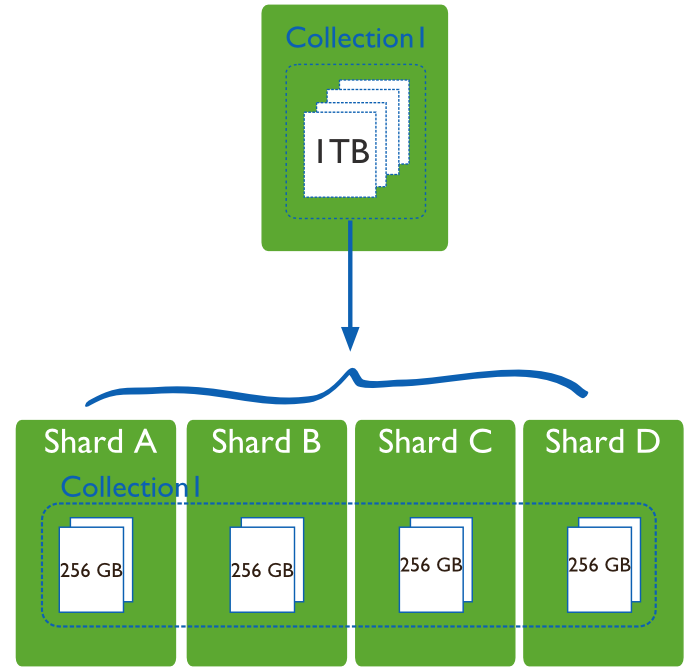
\includegraphics[width=0.8\linewidth]{sharded-collection.png}
\end{figure}
\end{columns}
\end{frame}


%------------------------------------------------
\begin{frame}
\frametitle{Caracteristicas}
\begin{columns}[c] % The "c" option specifies centered vertical alignment while the "t" option is used for top vertical alignment

\column{.45\textwidth} % Left column and width
\begin{enumerate}
\item Document-Oriented Storage
\item Full Index Support
\item Replication y High Availability
\item Auto Sharding
\item \textbf{Querying}
\item Map Reduce
\item GridFS
\item Other more...
\end{enumerate}

\column{.5\textwidth} % Right column and width
Gran cantidad de consultas basadas en los documentos.
\begin{example}[querys]
db.collection.find(\{\})
\\~\\
db.collection.find(\{'field':'jesse'\})
\\~\\
db.inventory.find().sort(\{field:1\})
\end{example}
\end{columns}
\end{frame}

%------------------------------------------------
\begin{frame}
\frametitle{Caracteristicas}
\begin{columns}[c] % The "c" option specifies centered vertical alignment while the "t" option is used for top vertical alignment

\column{.45\textwidth} % Left column and width
\begin{enumerate}
\item Document-Oriented Storage
\item Full Index Support
\item Replication y High Availability
\item Auto Sharding
\item Querying
\item \textbf{Map Reduce}
\item GridFS
\item Other more...
\end{enumerate}

\column{.5\textwidth} % Right column and width
Map Reduce es un paradigma de procesamiento de datos para condensar grandes volumenes de datos.
\begin{figure}
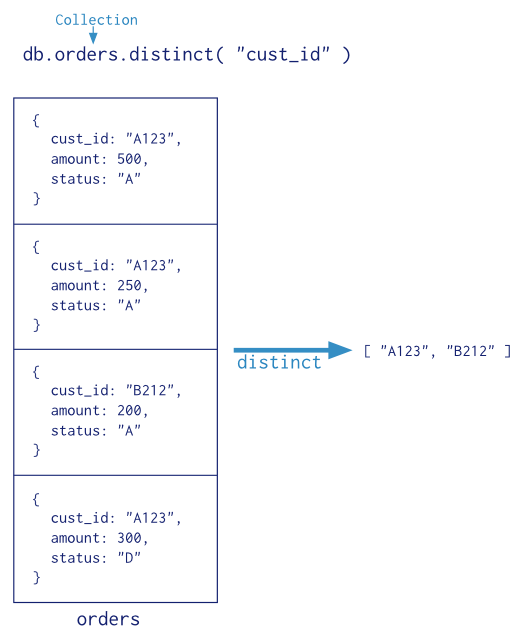
\includegraphics[width=0.5\linewidth]{distinct.png}
\end{figure}
\end{columns}
\end{frame}


%------------------------------------------------
\begin{frame}
\frametitle{Caracteristicas}
\begin{columns}[c] % The "c" option specifies centered vertical alignment while the "t" option is used for top vertical alignment

\column{.45\textwidth} % Left column and width
\begin{enumerate}
\item Document-Oriented Storage
\item Full Index Support
\item Replication y High Availability
\item Auto Sharding
\item Querying
\item Map Reduce
\item \textbf{GridFS}
\item Other more...
\end{enumerate}

\column{.5\textwidth} % Right column and width
GridFS es una especificaci\'on para almacenar y recuperar archivos que exceden el limite del tamano de 16MB en los documentos BSON.
\\~\\
util utillizarlo para almacenar imagenes, audio, video, archivos de texto, etc...
\end{columns}
\end{frame}


%------------------------------------------------
\begin{frame}
\frametitle{Caracteristicas}
\begin{columns}[c] % The "c" option specifies centered vertical alignment while the "t" option is used for top vertical alignment

\column{.45\textwidth} % Left column and width
\begin{enumerate}
\item Document-Oriented Storage
\item Full Index Support
\item Replication y High Availability
\item Auto Sharding
\item Querying
\item Map Reduce
\item GridFS
\item \textbf{Other more...}
\end{enumerate}

\column{.5\textwidth} % Right column and width
\begin{itemize}
\item MMS.
\item Partner with MongoDB.
\item Multiples drivers.
\end{itemize}

\end{columns}
\end{frame}


%------------------------------------------------
\begin{frame}
\frametitle{Instalacion}
\begin{columns}[c] % The "c" option specifies centered vertical alignment while the "t" option is used for top vertical alignment

\column{.50\textwidth} % Left column and width
\begin{block}{Terminal}
\begin{enumerate}
\item Statement
\item Explanation
\item Example
\end{enumerate}
\end{block}

%\column{.5\textwidth} % Right column and width
%\begin{block}{casa}
%\begin{enumerate}
%\item Statement
%\item Explanation
%\item Example
%\end{enumerate}
%\end{block}

\end{columns}
\end{frame}

%------------------------------------------------

\begin{frame}
\frametitle{SHELL}
\begin{columns}[c] % The "c" option specifies centered vertical alignment while the "t" option is used for top vertical alignment

\column{.45\textwidth} % Left column and width
\textbf{Heading}
\begin{enumerate}
\item Statement
\item Explanation
\item Example
\end{enumerate}

\column{.5\textwidth} % Right column and width
Lorem ipsum dolor sit amet, consectetur adipiscing elit. Integer lectus nisl, ultricies in feugiat rutrum, porttitor sit amet augue. Aliquam ut tortor mauris. Sed volutpat ante purus, quis accumsan dolor.

\end{columns}
\end{frame}

%------------------------------------------------

\begin{frame}
\frametitle{Insert Find Update Remove (CRUD)}
\begin{columns}[c] % The "c" option specifies centered vertical alignment while the "t" option is used for top vertical alignment

\column{.45\textwidth} % Left column and width
\textbf{Heading}
\begin{enumerate}
\item Statement
\item Explanation
\item Example
\end{enumerate}

\column{.5\textwidth} % Right column and width
Lorem ipsum dolor sit amet, consectetur adipiscing elit. Integer lectus nisl, ultricies in feugiat rutrum, porttitor sit amet augue. Aliquam ut tortor mauris. Sed volutpat ante purus, quis accumsan dolor.

\end{columns}
\end{frame}

%------------------------------------------------

\begin{frame}
\frametitle{DEMO =)}
\begin{columns}[c] % The "c" option specifies centered vertical alignment while the "t" option is used for top vertical alignment

\column{.45\textwidth} % Left column and width
\textbf{Heading}
\begin{enumerate}
\item Statement
\item Explanation
\item Example
\end{enumerate}

\column{.5\textwidth} % Right column and width
Lorem ipsum dolor sit amet, consectetur adipiscing elit. Integer lectus nisl, ultricies in feugiat rutrum, porttitor sit amet augue. Aliquam ut tortor mauris. Sed volutpat ante purus, quis accumsan dolor.

\end{columns}
\end{frame}

%------------------------------------------------

\begin{frame}
\frametitle{Administradores graficos}
\begin{columns}[c] % The "c" option specifies centered vertical alignment while the "t" option is used for top vertical alignment

\column{.45\textwidth} % Left column and width
\textbf{Heading}
\begin{enumerate}
\item Statement
\item Explanation
\item Example
\end{enumerate}

\column{.5\textwidth} % Right column and width
Lorem ipsum dolor sit amet, consectetur adipiscing elit. Integer lectus nisl, ultricies in feugiat rutrum, porttitor sit amet augue. Aliquam ut tortor mauris. Sed volutpat ante purus, quis accumsan dolor.

\end{columns}
\end{frame}


%------------------------------------------------
\section{MongoDB Medellin}
%------------------------------------------------

\begin{frame}
\frametitle{Comunidad}
\begin{table}
\begin{tabular}{l l l}
\toprule
\textbf{Treatments} & \textbf{Response 1} & \textbf{Response 2}\\
\midrule
Treatment 1 & 0.0003262 & 0.562 \\
Treatment 2 & 0.0015681 & 0.910 \\
Treatment 3 & 0.0009271 & 0.296 \\
\bottomrule
\end{tabular}
\caption{Table caption}
\end{table}
\end{frame}

%------------------------------------------------
\begin{frame}
\frametitle{Theorem}
\begin{theorem}[Mass--energy equivalence]
$E = mc^2$
\end{theorem}
\end{frame}

%------------------------------------------------

\begin{frame}
\frametitle{Figure}
Uncomment the code on this slide to include your own image from the same directory as the template .TeX file.
\begin{figure}
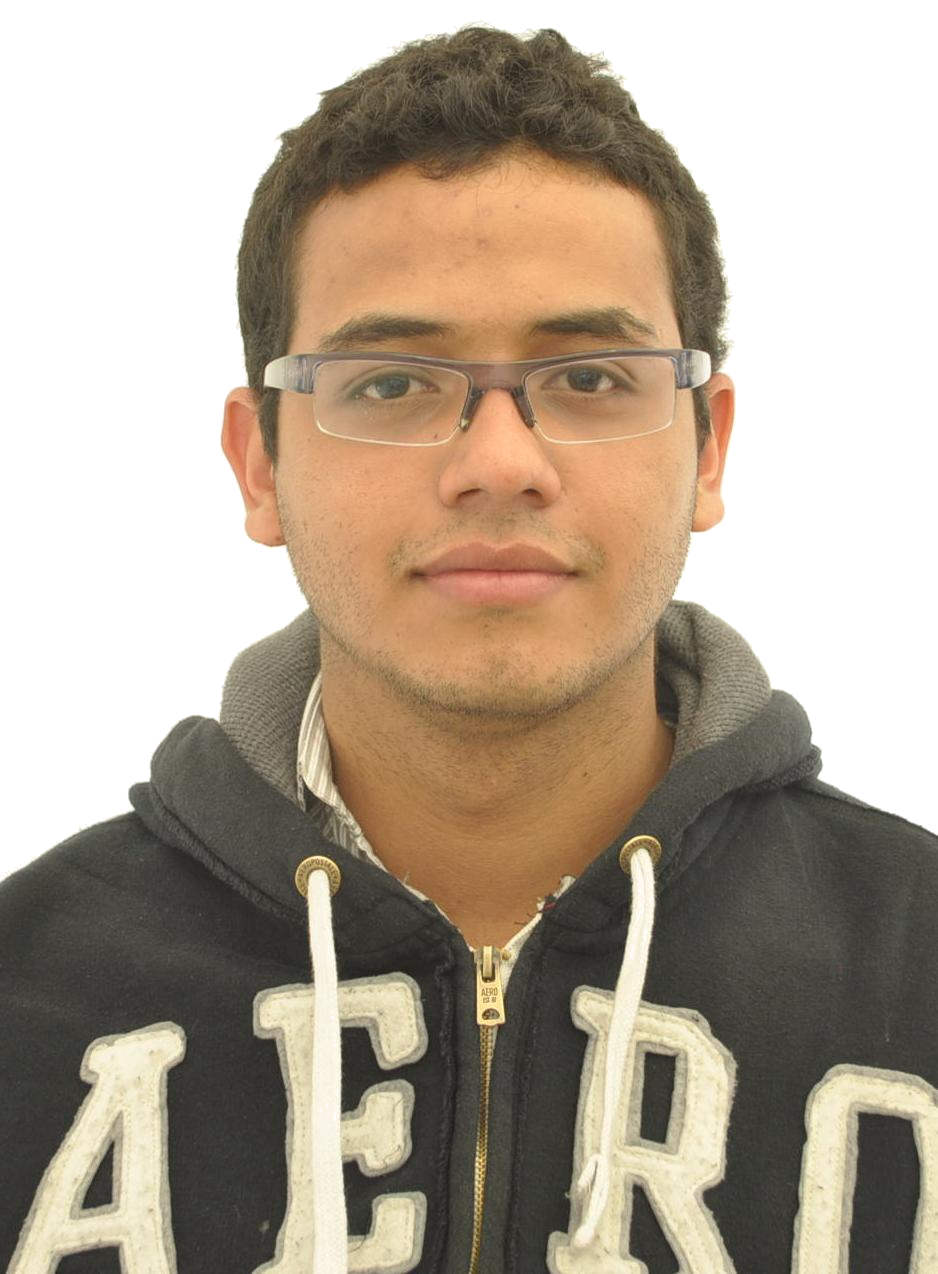
\includegraphics[width=0.1\linewidth]{JesseFoto.png}
\end{figure}
\begin{figure}
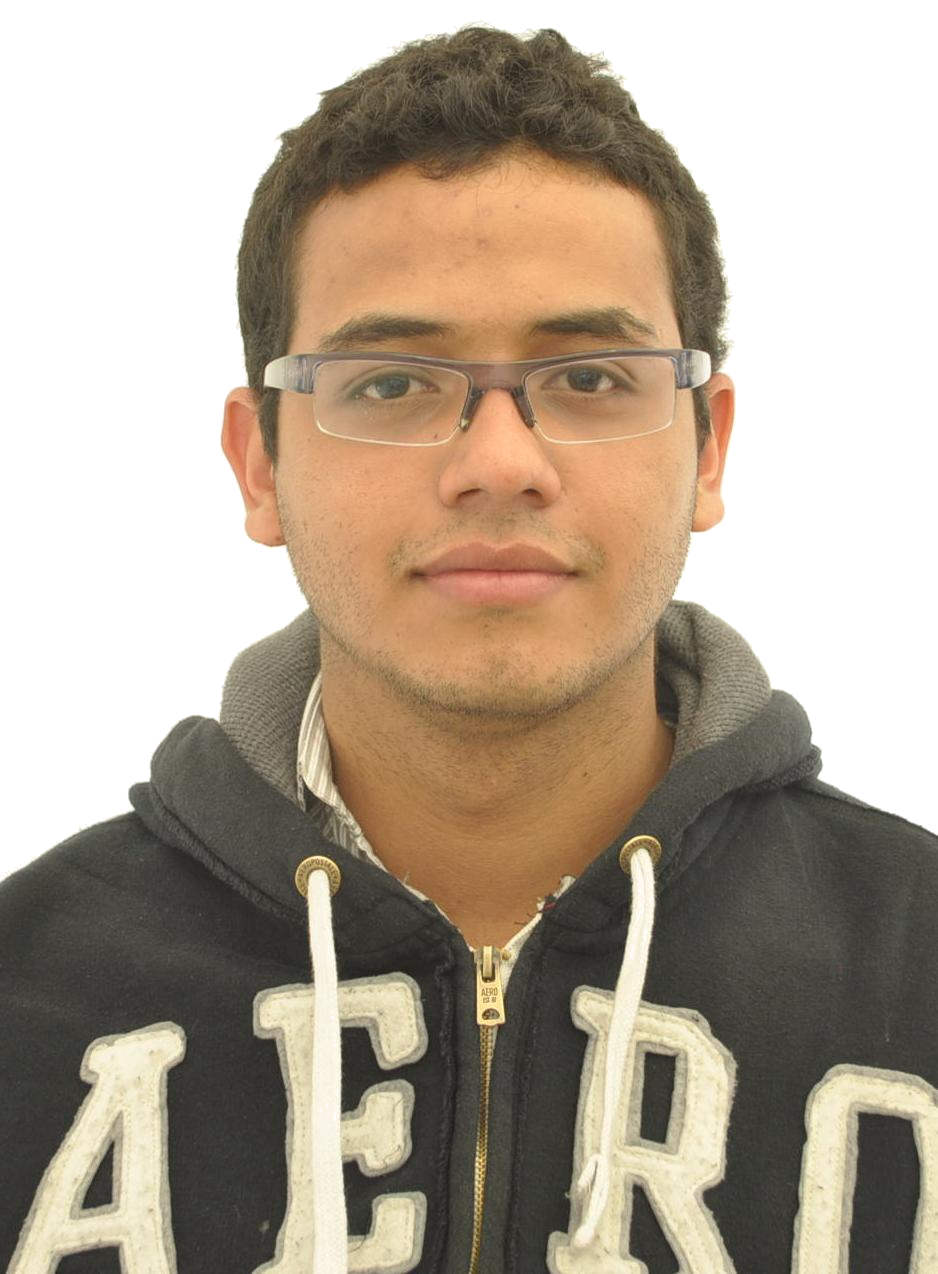
\includegraphics[width=0.2\linewidth]{JesseFoto.png}
\end{figure}
\end{frame}

%------------------------------------------------

\begin{frame}[fragile] % Need to use the fragile option when verbatim is used in the slide
\frametitle{Citation}
An example of the \verb|\cite| command to cite within the presentation:\\~

This statement requires citation \cite{p1}.
\end{frame}

%------------------------------------------------

\begin{frame}
\frametitle{References}
\footnotesize{
\begin{thebibliography}{99} % Beamer does not support BibTeX so references must be inserted manually as below
\bibitem[Smith, 2012]{p1} John Smith (2012)
\newblock Title of the publication
\newblock \emph{Journal Name} 12(3), 45 -- 678.
\end{thebibliography}
}
\end{frame}

%------------------------------------------------

\begin{frame}
\Huge{\centerline{Gracias !!! =)}}
\end{frame}

%----------------------------------------------------------------------------------------

\end{document} 
